\clearpage
\section{合成のしかたを選ぶ（設定の\ui{スタック}タブ）}\label{sec:stacking}

\begin{figure}[H]
\centering
\begin{screenshot}[0.46\linewidth]{settings_stack}
  \calloutleft{1}{tabs}
  \calloutleft{2}{mode}
  \calloutleft{3}{align}
  \calloutleft{4}{sigma}
  \calloutright{5}{mask}
  \calloutright{6}{lens}
  \calloutleft{7}{format}
  \calloutleft{8}{start}
  \calloutleft{9}{export}
\end{screenshot}
\caption{設定の\ui{スタック}タブ}
\end{figure}

\begin{callouts}
\co{1} \ui{スタック}・\ui{タイムラプス}：設定の画面を切り替えます。
\co{2} \textbf{スタック方式}：合成のしかたを選びます（下の表）。
\co{3} \ui{アライメント（星の位置合わせ）}：写真ごとの星のずれを合わせてから重ねます。
\co{4} \ui{シグマクリッピング}：飛行機や人工衛星の光などを取り除いてから平均します（\ref{sec:sigma}節）。平均のときだけ表示されます。
\co{5} \textbf{空と地上（新星景モード）}：空と地上を分けて合成します（\ref{sec:nightscape}節）。
\co{6} \textbf{レンズプロファイル}：DNG にレンズの情報を入れます（\ref{sec:export}節）。
\co{7} 書き出す形式を選びます（\ref{sec:export}節）。
\co{8} \ui{★ スタッキング開始}：合成を始めます。
\co{9} \ui{結果を書き出す…}：合成した結果を保存します。
\end{callouts}

\subsection{スタック方式}

\begin{center}
\small
\begin{tabularx}{\linewidth}{l X X}
\toprule
方式 & 結果 & こんなときに \\
\midrule
平均 (Average) & 全部の写真の平均。ノイズがいちばん減ります。 & ふつうはこれ。天の川や星雲をなめらかにしたいとき。 \\
中央値 (Median) & 画素ごとに、真ん中の値を使います。1枚だけに写った飛行機などが消えます。 & 飛行機や人工衛星がたくさん写ったとき。ただしノイズの減り方は平均より少なめで、メモリを多く使います。 \\
比較明合成 (Star Trails) & 画素ごとに、いちばん明るい値を残します。星が動いた跡が線になります。 & 星の軌跡（スタートレイル）を作りたいとき（\ref{sec:startrail}節）。 \\
\bottomrule
\end{tabularx}
\end{center}

\begin{hint}[中央値とシグマクリッピング]
飛行機や人工衛星の光を消したいときは、「平均＋シグマクリッピング」がおすすめです。平均と同じくらいノイズが減り、光跡も消せます。
\end{hint}

\subsection{アライメント（星の位置合わせ）}

星は時間とともに動くので、そのまま重ねると星がにじみます。\ui{アライメント}にチェックを入れると、写真に写った星だけを見つけて位置を合わせてから重ねます（地上の模様には合わせません）。

\begin{itemize}[itemsep=0.3ex]
  \item \textbf{平均・中央値}：最初からチェックが入っています。ふつうは入れたままにします。
  \item \textbf{比較明合成}：最初はチェックが外れています（星の軌跡を残すため）。チェックを入れると、星が線ではなく点になります。
\end{itemize}

\begin{caution}[地上の風景がにじむ]
星に合わせて重ねると、地上の風景は少しずつずれて重なるので、にじみます。星と地上の両方をくっきりさせたいときは、新星景モード（\ref{sec:nightscape}節）を使ってください。
\end{caution}

\subsection{シグマクリッピング}\label{sec:sigma}

\begin{figure}[H]
\centering
\begin{screenshot}[0.46\linewidth]{settings_sigma}
  \calloutleft{1}{sigma}
  \calloutbelow{2}{low}
  \calloutbelow{3}{high}
\end{screenshot}
\caption{シグマクリッピングの設定}
\end{figure}

\begin{callouts}
\co{1} \ui{シグマクリッピング（外れ値を除いて平均）}：チェックを入れると使います。
\co{2} \textbf{κ 下側}：ほかの写真より暗すぎる値を、どれくらいで外れ値とするか（1〜10、最初は 3.0）。
\co{3} \textbf{κ 上側}：ほかの写真より明るすぎる値を、どれくらいで外れ値とするか（1〜10、最初は 3.0）。
\end{callouts}

画素ごとに、ほかの写真と比べて明るさが大きく外れている値（飛行機・人工衛星の光、ホットピクセル、宇宙線など）を除いてから平均します。
κ（カッパ）を小さくするほど、少しの違いでも外れ値として除きます。ふつうは 3.0 のままで十分です。3枚以上の写真で使えます。

\begin{figure}[H]
\centering
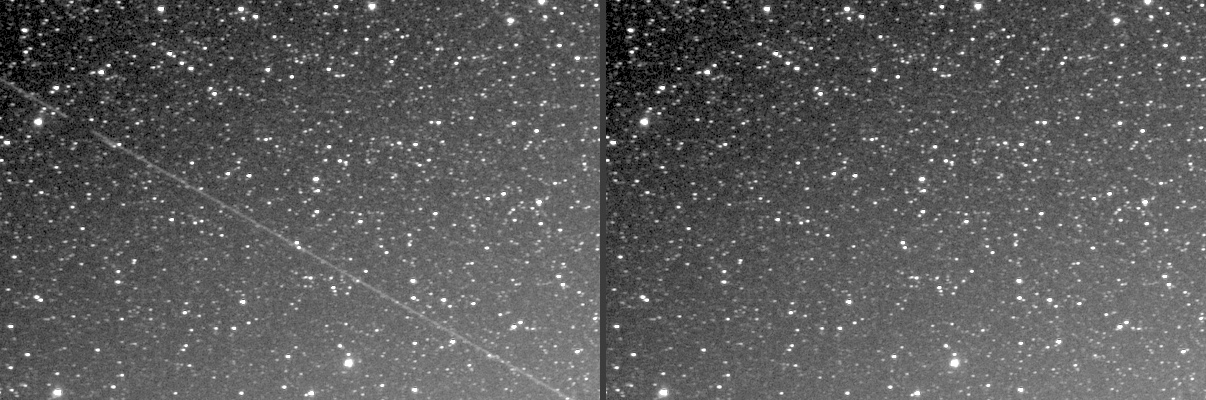
\includegraphics[width=0.9\linewidth]{figures/photo_sigma_trail}
\caption{シグマクリッピングの効果（左：ふつうの平均、右：シグマクリッピング）。人工衛星の光跡が消えます}
\end{figure}

\begin{caution}[流れる雲や明滅する灯り]
時間とともに変わるもの（流れる雲、明るさの変わる街の灯りなど）は、画素ごとに残る写真が変わるため、角張ったむらになることがあります。
気になるときは、シグマクリッピングを外してください。
\end{caution}

\begin{figure}[H]
\centering
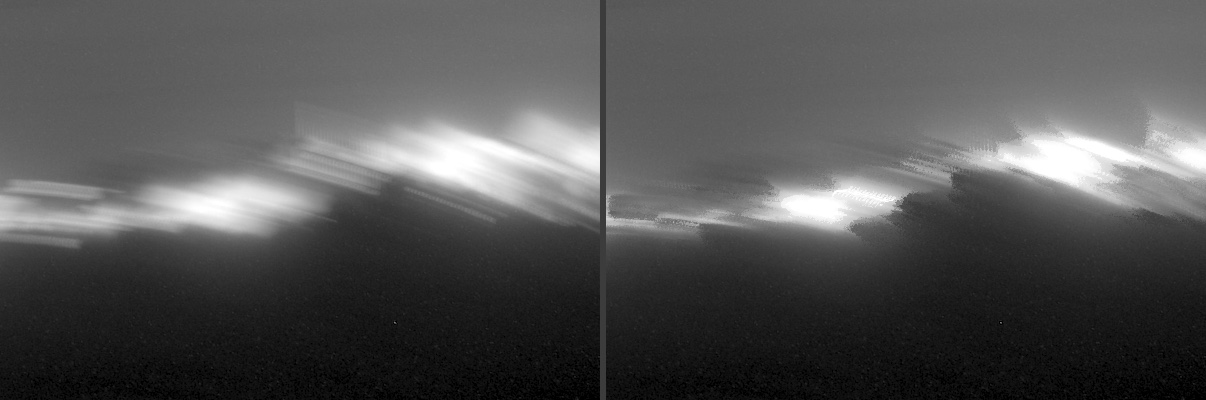
\includegraphics[width=0.9\linewidth]{figures/photo_sigma_cloud}
\caption{流れる雲と街の灯りの所（左：ふつうの平均、右：シグマクリッピング）。右では角張ったむらになっています}
\end{figure}
